\documentclass{article}
\usepackage[utf8]{inputenc}
\usepackage{amsmath}
\usepackage{natbib}
\usepackage{graphicx}
\usepackage[utf8]{inputenc}
\usepackage[english,russian]{babel}
\usepackage{cmap}
\usepackage{float}
\usepackage{amsmath,amssymb}

\begin{document}

\section{Домашняя работа №1}

\subsection{Задание 1}

С помощью $R[0,1]$ реализовать датчик распределения $Bi(5, \frac{1}{2})$. По смоделированным выборкам длины
100 и 100 000 построить на одном рисунке графики ряда частот и теоретический график. По выборкам
вычислить выборочные среднее и дисперсию, сравнить их с теоретическими значениями.

\subsubsection{Решение}
Для того, чтобы получить распределение $Bi(5, \frac{1}{2})$ из генератора $R[0,1]$, 
возьмем 5 генераторов и полим выборку размерности 5, то есть $X = (X_1, X_2, X_3, X_4, X_5)$, где
$X_i$ - случайная величина, причем $X_i \sim R[0, 1]$. 

Чтобы выполнялось второе условие, то есть "вероятность успеха $\frac{1}{2}$", выберем на отрезке
$[0, 1]$ точку $\frac{1}{2}$, тогда отрезок будет разделен на две равные части. Теперь будем
предпологать, что все значения на полуинтервале $[0, \frac{1}{2})$ 
соответствуют нулю, а $[\frac{1}{2}, 1]$ единице. Вернем сумму полученных генераторов, что
будет той самой случайной величиной $Y \sim Bi(5, \frac{1}{2})$

Рассмотрим графики полученного распределения.

\begin{figure}[h]
\center{
    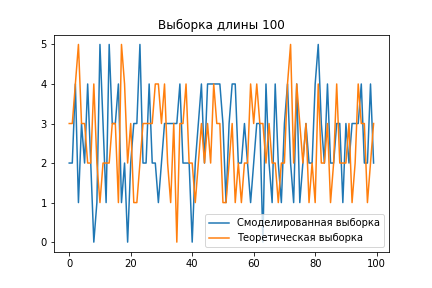
\includegraphics[scale=0.39]{./Task1/Task_1__all_100.png}
    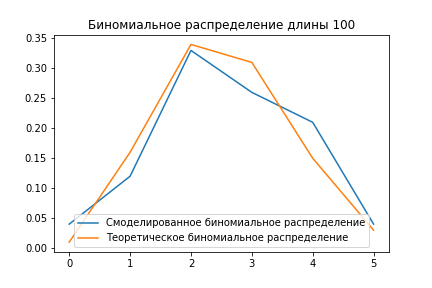
\includegraphics[scale=0.39]{./Task1/Task_1_Binom100.png}
    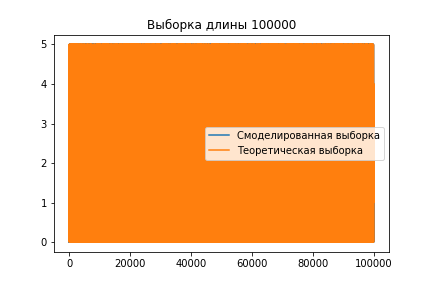
\includegraphics[scale=0.39]{./Task1/Task_1__all_100000.png}
    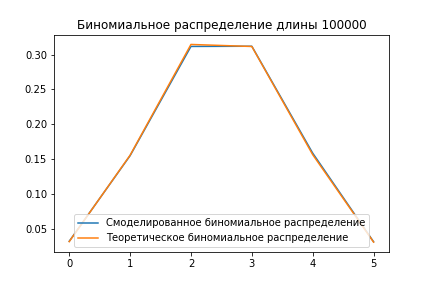
\includegraphics[scale=0.39]{./Task1/Task_1_Binom100000.png}
}
\caption{Распределение Бернулли}
\label{fig:image}
\end{figure}

Вычислим выборочное среднее:

    \[X = (X_1, X_2, ..., X_n); n = \{100, 100000\}; 
    \mathbb{E}_X = \sum_{i = 0}^{n}\frac{1}{n} * X_i\]

И дисперсию:
    \[X = (X_1, ..., X_n); n = \{100, 100000\};
    \mathbb{D}_X = \mathbb{E}_{X^2} - (\mathbb{E}_X)^2\]

Для выборки длины 100:
\begin{itemize}
    \item Выборочное среднее: $2.6$, теоретическое: $2.52$
    \item Дисперсия смоделированной выборки: $1.38$, теоретическое: $1.1095999999999995$
\end{itemize}

Для выборки длины 100000:
\begin{itemize}
    \item Выборочное среднее: $2.50395$, теоретическое: $2.498$
    \item Дисперсия смоделированной выборки: $1.2560643974999994$, теоретическое: $1.2472359999999991$
\end{itemize}

\subsection{Задание 2}
С помощью $R[0,1]$ реализовать датчик стандартного распределения Коши. По смоделированным выборкам длины 100 и 100 000 построить на одном рисунке теоретических и эмпирических функций распределения. На одном рисунке построить гистограммы смоделированных выборок (число и положение разрядов выбрать самостоятельно, но осмысленно!) и теоретическую плотность распределения. Вычислить выборочные медианы и сравнить их с теоретическим значением.

\subsubsection{Решение}
Для моделлирования случайных величин некоторого распределения через генератор 
равномерного распределение рассмотрим функцию, обратную функции распределения Коши: 
\[ F^{-1}(X) = \tg\left({\pi*(X-\frac{1}{2})}\right), X \sim R[0,1]\]
По решению задачи №7 полученная случайная величина $Y = F^{-1}(X)$ распределена 
по закону Коши, то есть $Y \sim C(0, 1)$. Для вычисления эмперической функции
распределения используем формулу:
\[F_n(x) = \frac{1}{n}*\sum_{k=1}^{n}I(x-X_k)\]

\begin{equation*}
    I(x)=
    \begin{cases}
        0 &\text{при $x \le 0$,}\\
        1 &\text{при $x < 0$.}
    \end{cases}
\end{equation*}

Для построения теоретического распределения воспользуемся распределением $C(0, 1)$:
\[F(x) = \frac{1}{\pi}*\arctg\left(x\right)+\frac{1}{2}\]

Рассмотрим полученные графики для выборки длины 100 и 100000:

\begin{figure}[h]
\center{
    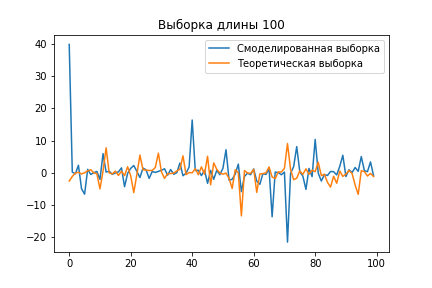
\includegraphics[scale=0.39]{./Task2/Task_2__all_100.png}
    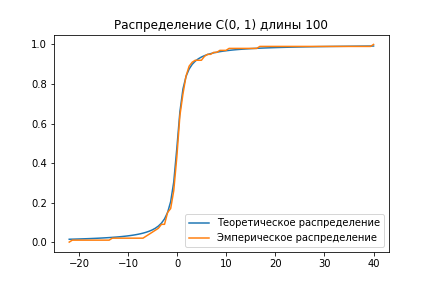
\includegraphics[scale=0.39]{./Task2/Task_2_Cauchy100.png}
    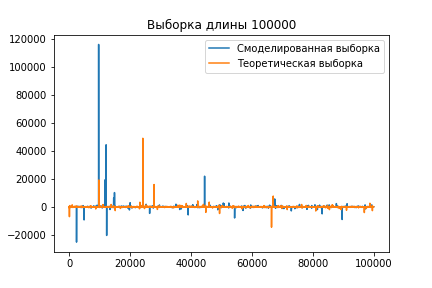
\includegraphics[scale=0.39]{./Task2/Task_2__all_100000.png}
    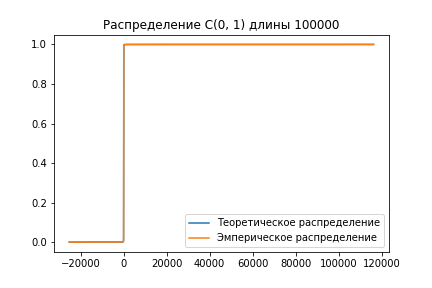
\includegraphics[scale=0.39]{./Task2/Task_2_Cauchy100000.png}
}
\caption{Распределение Коши}
\label{fig:image}
\end{figure}

Построим гистограмму и плотность распределения Коши. Для плотности справедлива формула:
\[f(x) = \frac{1}{\pi*\left(1+x^2\right)}\]

Чтобы построить гистограмму,  определим число разрядов и выберем отрезок так, чтобы
выполнялось условие нормировки. Данный вопрос рассмотрен в задаче №3, поэтому выберем отрезок
так, что левая границы соответствует минимуму из полученной выборки, а правая - максимуму:
\[X = \left(X_1, ..., X_n\right), [a,b] = \left[\min_{i \in \overline{1,n}}X_i,
\max_{i \in \overline{1, n}}{X_i}\right]\]

Для определения числа разрядов гистограммы воспользуемся правилом Стёрджеса. Число разрядов
$n$ определяется через размер выборки $N$:
\[n(N) = 1+\left\lfloor{\log_2N}\right\rfloor\]

Используя полученные значения, построим плотность и гистограмму распределения Коши:

\begin{figure}[h]
\center{
    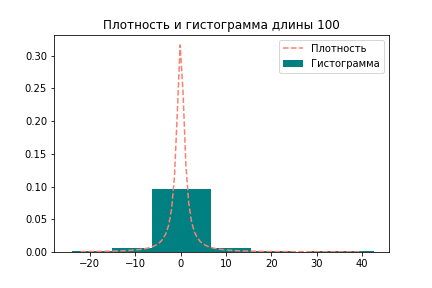
\includegraphics[scale=0.5]{./Task2/Task_2_Density100.png} 
    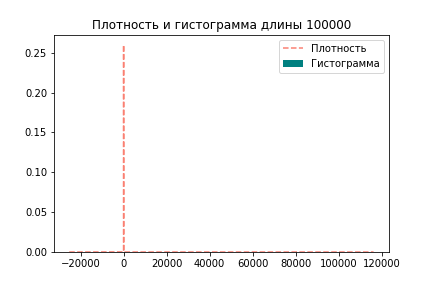
\includegraphics[scale=0.5]{./Task2/Task_2_Density100000.png}
}
\caption{Плотность и гистограмма распределения Коши}
\label{fig:image}
\end{figure}

Вычислим выборочную медиану и сравним значение с теоретическим аналогом. Теоретическое значение
получается при подстановке в обратную функцию распределения число $\frac{1}{2}$:

\[M = F^{-1}(\frac{1}{2})\]

\begin{itemize}
    \item Для выборки длины 100 выборочная медиана: 0.21787135837578478; Теоретическое значение: 0
    \item Для выборки длины 100000 выборочная медиана: -0.0005758960784728971; Теоретическое значение: 0
\end{itemize}

\subsection{Задание 3}
В условиях задачи 8 выбрать произвольную кусочно-постоянную плотность с 5 разрядами. 
помощью $R[0,1]$ реализовать соответствующий генератор. По смоделированным выборкам длины
1000 и 100 000 построить на одном рисунке теоретических и эмпирических функций
распределения. По выборкам вычислить выборочные среднее и дисперсию, сравнить их с 
теоретическими значениями. На одном рисунке построить гистограммы смоделированных выборок
и теоретическую плотность распределения. Разряды гистограмм выбирать двумя способами: 1)
совпадающими с теоретическими разрядами распределения, 2) разбивающими теоретические 
разряды пополам. По выборкам вычислить выборочные среднее и дисперсию, сравнить их с
теоретическими значениями.
\subsubsection{Решение}
Чтобы смоделировать кусочно-постоянную плотность распределения, рассмотрим отрезок 
$[0, 1]$. На данном отрезке возьмем 5 точек, не равных нулю, и ноль. Например:
\[[0, 1] \to \left[0, \frac{5}{16}\right) \cup \left[\frac{5}{16}, \frac{7}{16}\right)
\cup \left[\frac{7}{16}, \frac{10}{16}\right) \cup \left[\frac{10}{16},
\frac{11}{16}\right) \cup \left[\frac{11}{16}, 1\right) \]

Теперь мы получили разбиение отрезка на 5 частей. Выберем на каждом плотность так, чтобы
выполнялось условие нормировки. Положим, что:

\begin{equation*}
    f(x) =     
    \begin{cases}
        0 &\text{при $x < 0$,}\\
        1 &\text{при $0 \le x < \frac{5}{16}$,}\\
        \frac{1}{2} &\text{при $\frac{5}{16} \le x < \frac{7}{16}$,}\\
        \frac{2}{3} &\text{при $\frac{7}{16} \le x < \frac{10}{16}$,}\\
        2 &\text{при $\frac{10}{16} \le x < \frac{11}{16}$,}\\
        \frac{6}{5} &\text{при $\frac{11}{16} \le x < 1$,}\\
        0 &\text{при $1 \le x$.}
    \end{cases}
\end{equation*}

Проверим условие нормировки:
\[\int_{-\infty}^{+\infty}f(x)dx = \frac{5}{16}\times1+\frac{2}{16}\times\frac{1}{2}+
\frac{3}{16}\times\frac{2}{3}+\frac{1}{16}\times2+\frac{5}{16}\times\frac{6}{5}
= 1\]

Поэтому выбранное разбиение верное и у полученной случайной величины кусочно-постоянная плотность. 
Чтобы смоделировать генератор полученной случайной величины используем два генератора
\begin{itemize}
    \item Первый генератор выдаст точку на отрезке $[0, 1]$. Используем наше разбиение отрезка на
        5 частей и определим, какому множеству принадлежит полученная точка
    \item Второй генератор покажет на какую позицию разбиения попадет точка. Уже
        определено, какому отрезку принадлежит данная точка, известна длина отрезка и значение
        левой границы. Найденные значения подставим в формулу случайной величины:
        \[X() = \sum_{i = 1}^5|X_i - X_{i-1}|*I_{\Delta\left[X_{i-1}, X_{i}\right]},
        X_0 = 0\]
\end{itemize}

Например, если после работы первого генератора точка находится на множестве $\left[0,
\frac{5}{16}\right)$, то позиция точки принадлежит этому же интервалу, тогда второй генератор
дает число от 0 до 1, которое умножается на длину замыкания данного множества, то есть на
$\frac{5}{16}$, затем прибавляется начало множества - точка 0. 

По определению распределения получим, что
\[F_X(x) = \int_{-\infty}^xf(x)dx\]

Так как плотность кусочно-постоянная, то функция распределения будет линейной функцией с
множителями перед $x$, соответствующими значению плотности на данном множестве, сложенная с
константой, равной $\int_{-\infty}^{a_l}f(x)dx$, где $a_l$ - левая граница данного множества.

Так как в точке $\frac{7}{16}$ плотность меняется с $\frac{1}{2}$ на $\frac{2}{3}$, для большей
наглядности добавленая вспомогательная функция $y(x) = \frac{2}{3}*x+\frac{1}{12}$,
показывающая, что перелом в точке $\frac{7}{16}$, хоть и незначительный, есть.

Для эмперической функции распределения используем уже упомянутую в предыдущих заданиях этого
документа формулу. Получим:

\begin{figure}[h]
\center{
    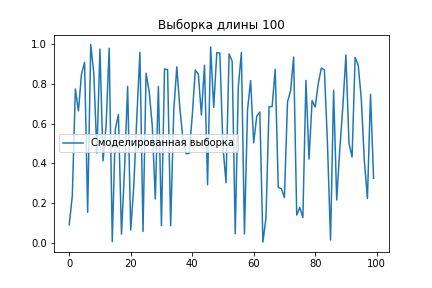
\includegraphics[scale=0.39]{./Task3/Task_3__all_100.png}
    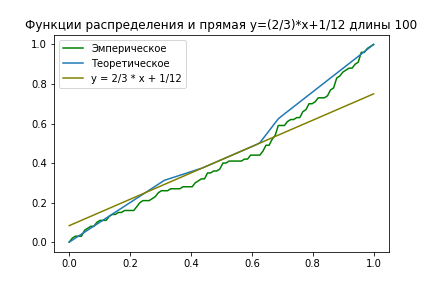
\includegraphics[scale=0.39]{./Task3/Task_3__distrib_100.png}
    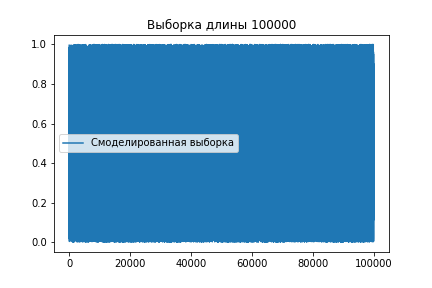
\includegraphics[scale=0.39]{./Task3/Task_3__all_100000.png}
    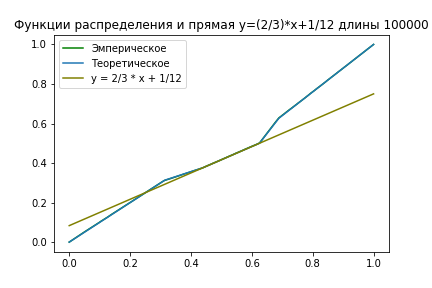
\includegraphics[scale=0.39]{./Task3/Task_3__distrib_100000.png}
}
\caption{Распределение с кусочно-постоянной плотностью}
\label{fig:image}
\end{figure}

Сравним полученные выборочные среднее и дисперсию, сравним их с еоретическими значениями:
\begin{itemize}
    \item Для выборки длины 100 выборочное среднее составило: 0.4252; теоретическое - 0.4632670454545454
    \item Для выборки длины 100000 выборочное среднее составило: 0.4633432522;
        теоретическое - 0.462890996097461
    \item Для выборки длины 100 выборочная дисперсия составила: 0.07501495999999996;
        теоретическая - 0.07843229629324083
    \item Для выборки длины 100000 выборочная дисперсия составила: 0.0766235435949392;
        теоретическая - 0.07666826120296805
\end{itemize}

При построении гистограммы использовалось два способа, как описано в условии задачи. 
Плотность данной случайной величины, как следует из требования задачи, кусочно-постоянная функция с
значениями указанными ранее на множествах описанных выше. Число разрядов фиксированно и в 1-ом
случае равно 5(по условию задачи), во втором случае равно 10.

Для построения гистограммы использовалась описанная ранее в заданиях этого документа формула.
Для выбора отрезка, на котором строится гистограмма, использовалась ранее описанная идея с
максимумом и минимумом выборки. Получим:

\begin{figure}[h]
\center{
    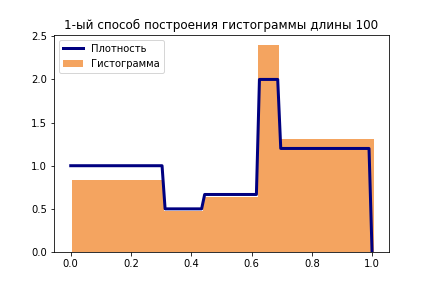
\includegraphics[scale=0.39]{./Task3/Task_3__density1_100.png}
    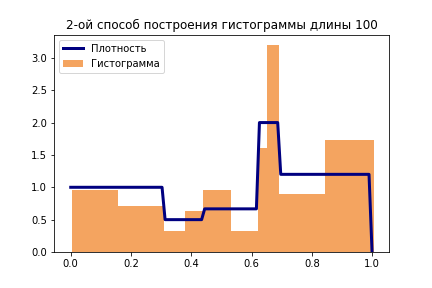
\includegraphics[scale=0.39]{./Task3/Task_3__density2_100.png}
    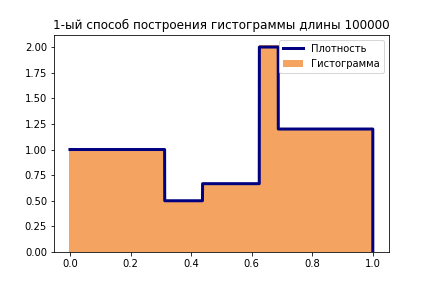
\includegraphics[scale=0.39]{./Task3/Task_3__density1_100000.png}
    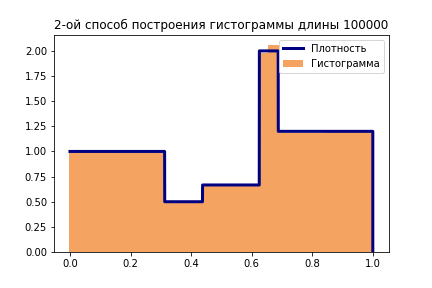
\includegraphics[scale=0.39]{./Task3/Task_3__density2_100000.png}
}
\caption{Плотность и гистограмма распределения с кусочно-постоянной плотностью}
\label{fig:image}
\end{figure}

\subsection{Задание 4}
В условиях задач 9 и 10 построить соответствующие генераторы $N(0,1)$. По смоделированным выборкам длины 
100 и 100 000 построить на одном рисунке теоретических и эмпирических функций распределения. Сравнить 
время генерации большой выборки 1-м и 2-м способом. На одном рисунке построить гистограммы смоделированных
 выборок и теоретическую плотность распределения (число и положение разрядов выбрать 
самостоятельно, но осмысленно!). Вычислить выборочные среднее, медиану, дисперсию, коэффициент 
асимметрии и куртозис. Сравнить полученные оценки с теоретическими. 

\subsubsection{Решение}
Чтобы смоделировать случайную величину воспользуемся формулами задач 9 и 10. В задаче 9 говорится, что 
$Y \sim N(0, 1)$, если 
\[Y = \sum_{k = 1}^{12}X_k - 6, X_i \sim R[0, 1]\]

В задаче 10 говорится, что $Y_1, Y_2 - \text{НОРСВ}, \text{ причем } Y_1, Y_2 \sim N(0, 1)$, если 
\[Y_1 = \sqrt{-2\ln{X_1}}*\sin{2\pi X_2}\]
\[Y_2 = \sqrt{-2\ln{X_1}}*\cos{2\pi X_2}; X_1, X_2 \sim R[0, 1]\]

Для построения эмперической функции распределения воспользуемся ранее описанной формулой. Чтобы построить теоретическую функцию распределения $N(0, 1)$ воспользуемся формулой:
\[\Phi(x) = \frac{1}{\sqrt{2\pi}}\int_{-\infty}^{x}e^{-\frac{t^2}{2}}dt\]

Рассмотрим функцию ошибок:
\[erf(x) = \frac{2}{\sqrt{\pi}}\int_{0}^{x}e^{-t^2}dt\]

Тогда, так как 
\[\int_{-\infty}^{0}e^{-\frac{t^2}{2}}dt = \left|\text{ в силу четности } e^{-\frac{t^2}{2}}\right| = \] 
\[=\int_{0}^{+\infty}e^{-\frac{t^2}{2}}dt = \left|u = \frac{t}{\sqrt{2}}\right| = 
\sqrt{2}*\int_{0}^{+\infty}e^{-u^2}du = \sqrt{2}*\frac{\sqrt{\pi}}{2}\]

Получаем, что 

\[F(x) = \Phi(\frac{x-0}{1}) = \Phi(x) = \frac{1}{\sqrt{2\pi}}\left(\int_{-\infty}^{0}e^{-\frac{t^2}{2}}dt + \int_{0}^{x}e^{-\frac{t^2}{2}}dt\right) = \]

\[=\left|u =\frac{t}{\sqrt{2}}; t = x => u = \frac{x}{\sqrt{2}}\right|=
\frac{\sqrt{2\pi}}{2*\sqrt{2\pi}}+\frac{\sqrt{2}}{\sqrt{2\pi}}\int_{0}^{\frac{x}{\sqrt{2}}}e^{-u^2}du=\]
\[\frac{1}{2}+\frac{1}{2}*\frac{2}{\sqrt{\pi}}\int_{0}^{\frac{x}{\sqrt{2}}}e^{-u^2}du = 
\frac{1}{2} + \frac{1}{2}*erf\left(\frac{x}{\sqrt{2}}\right) = \]
\[= \frac{1}{2}\left(1+erf\left(\frac{x}{\sqrt{2}}\right)\right)\]

Получим график теоретических и эмперических функций распределения:

\begin{figure}[h]
	\center{
		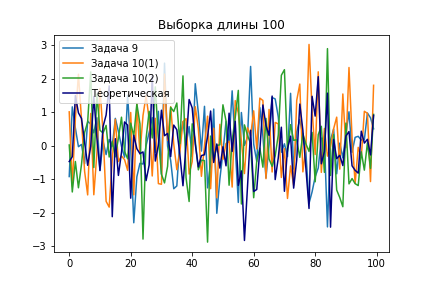
\includegraphics[scale=0.39]{./Task4/Task_4__all_100.png}
		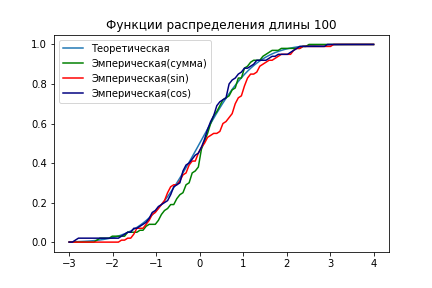
\includegraphics[scale=0.39]{./Task4/Task_4__distrib_100.png}
		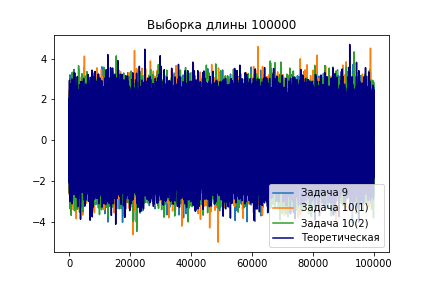
\includegraphics[scale=0.39]{./Task4/Task_4__all_100000.png}
		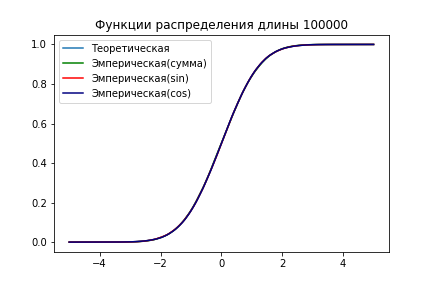
\includegraphics[scale=0.39]{./Task4/Task_4__distrib_100000.png}
	}
	\caption{Эмперическое и теоретическое распределение $N(0, 1)$}
	\label{fig:image}
\end{figure}

Для построения гистограмм будем использовать описанное выше правило Стёрджеса, но ограничим максимальное число разрядов 13-ью для большего сходства с функцией плотности распределения $N(0, 1)$. Получим:

\begin{figure}[H]
	\center{
		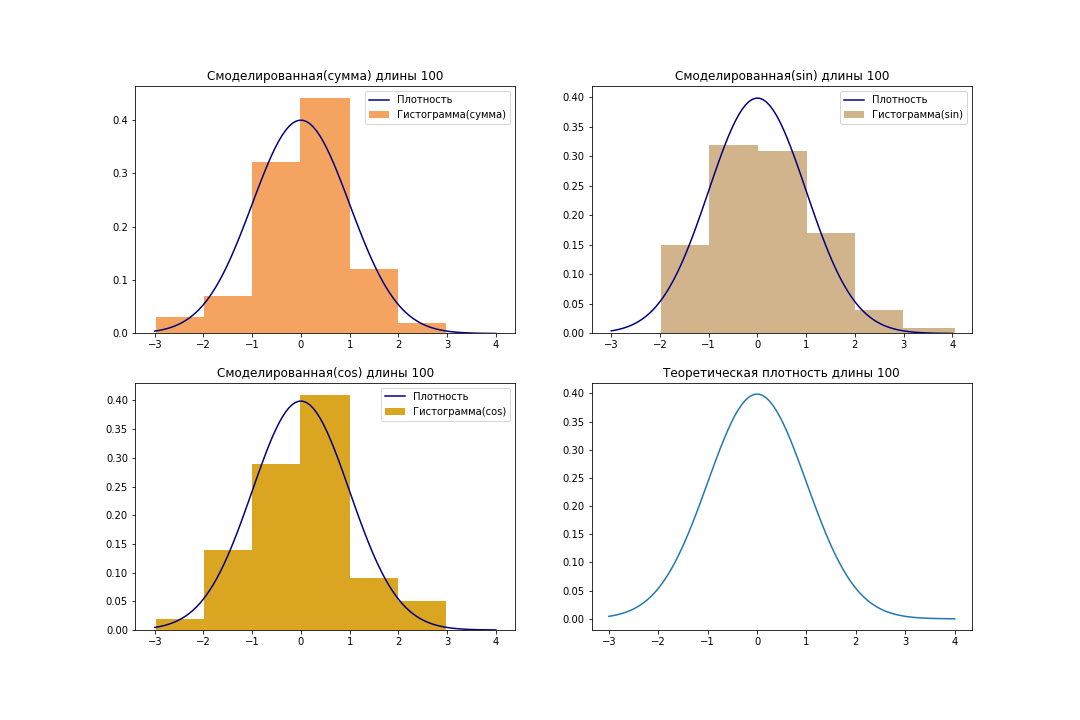
\includegraphics[scale=0.39]{./Task4/Task_4__gist&density_100.png}
		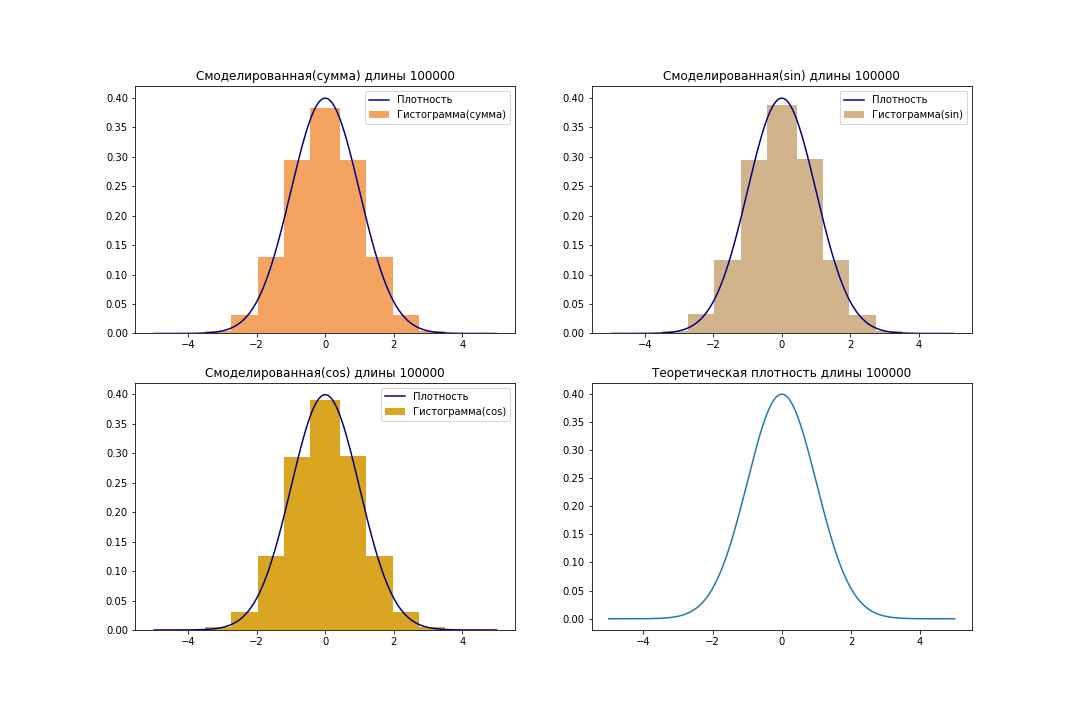
\includegraphics[scale=0.39]{./Task4/Task_4__gist&density_100000.png}
	}
	\caption{Гистограмма и плотность распределения $N(0, 1)$}
	\label{fig:image}
\end{figure}

Вычислим выборочные среднее, медиану, димперсию, коэффициент асимметрии и куртозис выборок и сравним значения с теоретическими. Чтобы получить значение коэффициента асимметрии и куртозиса(точки эксцесса) воспользуемся 3-им и 4-ым центральными моментами, соответственно:
\[\mu_3 = \mathbb{E}\left[\left(X - \mathbb{E}X\right)^3\right]; 
\mu_4 = \mathbb{E}\left[\left(X - \mathbb{E}X\right)^4\right]\]

Тогда коэфициент асимметрии вычисляется по формуле:
\[\gamma_1 = \frac{\mu_3}{\sigma^3}, \text{ где } \sigma = \sqrt{\mathbb{D}X}\]

Куртозис(коэффициент эксцесса) вычисляется по формуле:
\[\gamma_2 = \frac{\mu_4}{\sigma^4} - 3, \text{ где } \sigma = \sqrt{\mathbb{D}X}\]
\begin{itemize}
	\item Для выборки длины 100:
	\begin{itemize}
		\item Выборочное среднее:
		\begin{itemize}
			\item Смоделированной способом из задачи 9: 0.0910158168777063
			\item Смоделированной способом из задачи 10($\sin$): 0.1654934183883899
			\item Смоделированной способом из задачи 10($\cos$): -0.0026908354182544948
			\item Теоретическое значение: -0.012619596910858977
		\end{itemize}
		\item Медиана:
		\begin{itemize}
			\item Смоделированной способом из задачи 9: 0.07708387887182333
			\item Смоделированной способом из задачи 10($\sin$): 0.06745237856342444
			\item Смоделированной способом из задачи 10($\cos$): 0.057021514761033974
			\item Теоретическое значение: -0.02203385002181522
		\end{itemize}
		\item Дисперсия:
		\begin{itemize}
			\item Смоделированной способом из задачи 9: 0.8226822193356137
			\item Смоделированной способом из задачи 10($\sin$): 1.1060584102999171
			\item Смоделированной способом из задачи 10($\cos$): 1.0443862099776926
			\item Теоретическое значение: 0.8772570659152759
		\end{itemize}
		\item Коэффициент асимметрии:
		\begin{itemize}
			\item Смоделированной способом из задачи 9: -0.191480781474908
			\item Смоделированной способом из задачи 10($\sin$): 0.19513689131670858
			\item Смоделированной способом из задачи 10($\cos$): 0.03550436729861416
			\item Теоретическое значение: -0.21989510241995067
		\end{itemize}
		\item Коэффициент эксцесса:
		\begin{itemize}
			\item Смоделированной способом из задачи 9: 0.5336327294441223
			\item Смоделированной способом из задачи 10($\sin$): -0.6135627930553267
			\item Смоделированной способом из задачи 10($\cos$): 0.6119197109455063
			\item Теоретическое значение: 0.295581227041471
		\end{itemize}
	\end{itemize}
\item Для выборки длины 100000:
\begin{itemize}
	\item Выборочное среднее:
	\begin{itemize}
		\item Смоделированной способом из задачи 9: -0.0023363939452022016
		\item Смоделированной способом из задачи 10($\sin$): -0.0006843351339917403
		\item Смоделированной способом из задачи 10($\cos$): -0.0005595550966315507
		\item Теоретическое значение: 0.0013744061430496612
	\end{itemize}
	\item Медиана:
	\begin{itemize}
		\item Смоделированной способом из задачи 9: -0.0025890223220645936
		\item Смоделированной способом из задачи 10($\sin$): 0.004607519065085341
		\item Смоделированной способом из задачи 10($\cos$): -0.0019349844763608373
		\item Теоретическое значение: 0.0013596938938788272
	\end{itemize}
	\item Дисперсия:
	\begin{itemize}
		\item Смоделированной способом из задачи 9: 0.9977870401191214
		\item Смоделированной способом из задачи 10($\sin$): 1.0011963348072879
		\item Смоделированной способом из задачи 10($\cos$): 0.9979599854898414
		\item Теоретическое значение: 0.9963919481329188
	\end{itemize}
	\item Коэффициент асимметрии:
	\begin{itemize}
		\item Смоделированной способом из задачи 9: -0.00645681214278904
		\item Смоделированной способом из задачи 10($\sin$): -0.006933815628778138
		\item Смоделированной способом из задачи 10($\cos$): -0.005617642448843749
		\item Теоретическое значение: -0.003866270917544823
	\end{itemize}
	\item Коэффициент эксцесса:
	\begin{itemize}
		\item Смоделированной способом из задачи 9: -0.114526076724503
		\item Смоделированной способом из задачи 10($\sin$): 0.0014470163841445
		\item Смоделированной способом из задачи 10($\cos$): 0.001145745622073
		\item Теоретическое значение: 0.012138581085752
	\end{itemize}
\end{itemize}
\end{itemize}

Сравним время генерации выборок способами из задачи 9 и задачи 10:
\begin{itemize}
	\item Для выборки длины 100
	\begin{itemize}
		\item Смоделированной способом из задачи 9: \\0.0008115768432617188 с
		\item Смоделированной способом из задачи 10($\sin$): \\0.0004260540008544922 с
		\item Смоделированной способом из задачи 10($\cos$): \\0.00045609474182128906 с
	\end{itemize}
	\item Для выборки длины 10000000
	\begin{itemize}
		\item Смоделированной способом из задачи 9: \\1.077580213546753 с
		\item Смоделированной способом из задачи 10($\sin$): \\0.4227886199951172 с
		\item Смоделированной способом из задачи 10($\cos$): \\0.41922783851623535 с
	\end{itemize}
\end{itemize}

\end{document}

